\documentclass[12pt]{article}

\usepackage[utf8]{inputenc}
\usepackage[T1]{fontenc}

% clickable links in pdf
\usepackage{hyperref}

% make title variable available
\usepackage{titling}

% create own header footer
\usepackage{fancyhdr}

% images
\usepackage{graphicx}

% grafics powerfull and hard
\usepackage{tikz}

% character spacing to fill line
\usepackage{microtype}

% image placement with [H]
\usepackage{float}

% fancy quotes
\usepackage{epigraph}

% extra symbols
\usepackage{textcomp}

% display code
\usepackage{listings}

% tables
\usepackage{tabu}
\usepackage{array}

% icons
\usepackage{fontawesome}


% make code copyable
\lstset{
upquote=true,
columns=fullflexible,
literate={*}{{\char42}}1
         {-}{{\char45}}1
}

\newsavebox{\picbox}

\graphicspath{ {./images/} }

% command for rounded corners
\newcommand{\cutpic}[3]{
  \savebox{\picbox}{\includegraphics[width=#2]{#3}}
  \tikz\node [draw, rounded corners=#1, line width=4pt,
    color=white, minimum width=\wd\picbox,
    minimum height=\ht\picbox, path picture={
      \node at (path picture bounding box.center) {
        \usebox{\picbox}};
    }] {};}


\title{
  \Huge
  \textbf{Globalizer} \\
  \vspace{0.2cm}
  \LARGE
  Anforderungsspezifikationen
}

\date{25.10.2018}
\author{
  Jonas Koller \\
  Donato Wolfisberg
}

\pagestyle{fancy}
\fancyhf{}
\rhead{\thedate}
\lhead{Globalizer Anforderungsspezifikationen}
\rfoot{\thepage}
\lfoot{Jonas Koller \& Donato Wolfisberg}


\begin{document}
  \begin{titlepage}
    \pagenumbering{gobble}

    \begin{center}
      \vspace*{-2cm}
      \cutpic{0.8cm}{4cm}{logo.jpg}

      \thetitle

      \vspace{2cm}

      \textbf{\theauthor}
    \end{center}

    \vfill

    \begin{figure}[H]
        \makebox[\linewidth]{
            
\includegraphics[width=1.3\linewidth]{globe.jpg}
        }
        \vspace*{-3cm}
    \end{figure}
  \end{titlepage}

  \newpage
  \pagenumbering{Roman}

  \begin{center}
    \makebox[\textwidth]{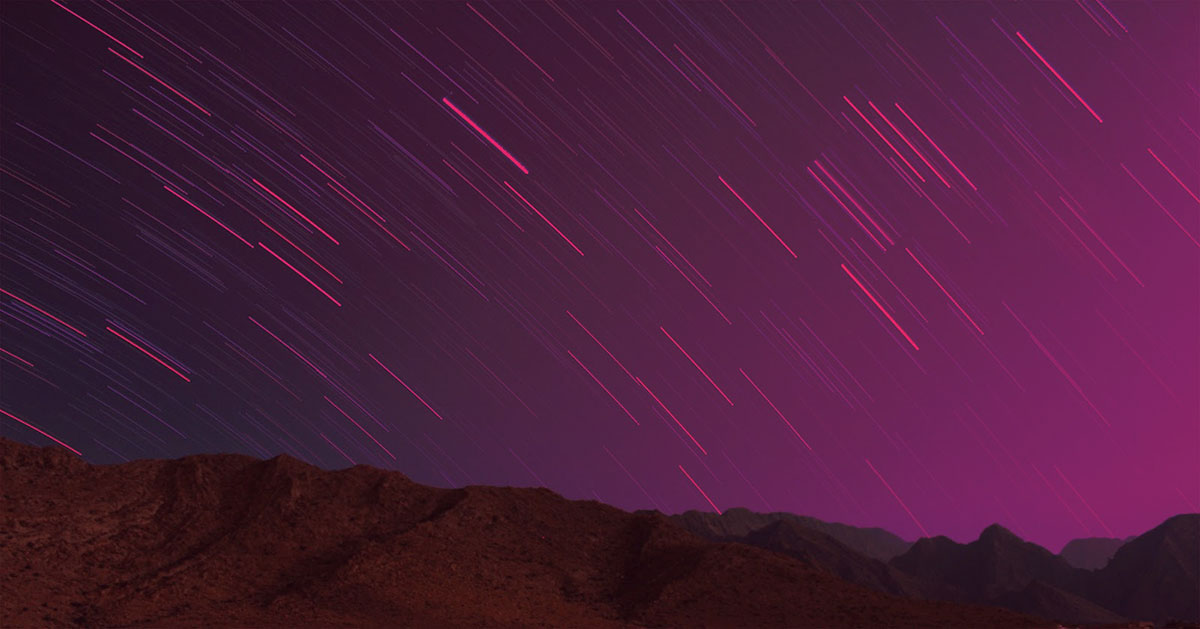
\includegraphics[width=\paperwidth]{nightsky.jpg}}
  \end{center}

  \section{Zweck des Dokuments}
    In diesem Dokument werden wir die Anforderungen an unser Projekt “Globalizer”.
    Das Projekt gilt im aktuellen Zustand als angenommen,
    da der Projektantrag durch Herr Manfred Rötheli angenommen wurde. Wir werden be\-schreiben,
    welche Anforderungen wir erfüllen möchten (“soll”-Anforderungen) und welche optionalen
    “kann”-Anforderungen wir eventuell auch erfüllen können.
    Es soll eine Übersicht für unser Vorhaben sein. Weiter sollen unsere Prozesse
    so gut wie möglich durch Grafiken dargestellt und visualisiert werden.
    Bei Fragen wenden sie sich an den Projektleiter (jonas.koller@gmx.ch).

  \section{Allgemeine Informationen}
    Hier folgt eine kurze Auflistung der Informationen zu diesem Dokument,
    dem Entwicklungsteam und dem aktuellen Stand.

  \subsection{Projektmitarbeiter}
    \begin{tabu} to \textwidth  {|l|l|X|l|}
      \hline
      \textbf{Name} & \textbf{Vorname}  & \textbf{E-Mail}                & \textbf{Funktion}     \\ \hline
      Koller        & Jonas             & jonas.koller@gmx.ch            & Projektleiter         \\ \hline
      Wolfisberg    & Donato            & donato.wolfisberg@gmail.com    & Entwickler            \\ \hline
      Gian          & Ott               & gian\_ott@sluz.ch              & Prüfer                \\ \hline
      Manuel        & Troxler           & manuel\_troxler@sluz.ch        & Prüfer                \\ \hline
    \end{tabu}

  \subsection{Änderungskontrolle}
    \begin{tabu} to \textwidth  {|l|l|l|X|}
      \hline
      \textbf{Version} & \textbf{Datum} & \textbf{Ausführende Stelle}     & \textbf{Funktion}                                 \\ \hline
      1                & 21.09.2018     & Projektteam                     & Erste Version \newline des Dokuments erstellt     \\ \hline
    \end{tabu}

  \subsection{Prüfung}
    \begin{tabu} to \textwidth  {|l|l|l|X|l|}
      \hline
      \textbf{Version} & \textbf{Datum} & \textbf{Ausführende Stelle}   & \textbf{Erreichter \newline Status}  & \textbf{Visum}  \\ \hline
                       &                &                               &                             &                 \\ \hline
    \end{tabu}

  \newpage
  \tableofcontents
  \newpage

  \pagenumbering{arabic}


  \section{Gesamtüberblick}
    \subsection{Allgemeine Beschreibung}
      Der Auftraggeber will für die Schule BBZW Sursee eine Chat Applikation entwickeln lassen.
      Für die Kommunikation zwischen den Schülern wie auch zum Lehrer. Es ist ihm wichtig dass
      die Anwender der Applikation komplett Anonym bleiben können. Die Applikation soll
      Modern und schnell als Webseite daher kommen und sowohl im Browser als auch
      auf mobilen Geräten funktionieren.

    \subsection{Ziele}
      Die Chat Applikation soll folgende Eigenschaften haben.

      \begin{enumerate}
        \item Anonymität der Anwender: Die Benutzer können sich Anonym auf der Applikation aufhalten.
          Da keinerlei Informationen vom Benutzer gespeichert werden sind auch automatisch
          die Anforderungen an den Datenschutz erfüllt.
        \item Modernes Design: Das Ziel besteht aus jungen Menschen die Gewohnt sind mit
          Informatik Instrumenten Arbeiten. Das erhöht die Akzeptanz der Anwendung.
        \item Kostengünstiger Betrieb: Der Auftraggeber verfügt nur über ein minimales Budget
          sodass die Applikation mit geringen Unterhalt und Hosting kosten auskommen muss.
        \item Hohe Verfügbarkeit: Die Applikation sollte eine Verfügbarkeit von 99\% haben,
          ohne dass ein Administration betrieben werden muss.
        \item Geschwindigkeit: Eine Chat Applikation beruht auf einem ständigen fragen und antworten. \newline
          Daher muss die Applikation sehr schnell sein.
      \end{enumerate}

    \subsection{Spezielle Aspekte}
      Weil die Applikation auf Anonymität beruht werden wir weder Ip Adressen noch Persönliche daten speichern,
      haben wir auch keine Sensible Nutzerdaten die wir noch speziell schützen müssten.

  \section{Analyse des IST-Systems}
    Es ist bis jetzt noch kein System vorhanden. Wir können alles von vorne Entscheiden.

  \section{Zielkatalog}
    In diesem Kapitel werden die Voraussetzungen an unser System genannt.

    \subsection{Beschreibung des SOLL-Systems}
      \subsubsection{Aktivitätsdiagramm}
        Bild wird noch übernommen
      \subsubsection{Externes Use Case Diagramm}
        Bild wird noch übernommen
      \subsubsection{Internes Use Case Diagramm}
        Bild wird noch übernommen

    \subsection{Zielsetzungen}
      \subsubsection{Muss-Ziele}
        \begin{enumerate}
          \item \faGlobe~ Globalen Gruppen Chat
          \item \faUser~ Hinterlegen eines Benutzernamens
          \item \faKey~ Session Anmeldung über UserKey
          \item \faMobile~ PWA
        \end{enumerate}

      \subsubsection{Kann-Ziele}
        \begin{enumerate}
          \item \faUsers~ Private Chats zwischen zwei Personen
          \item \faGoogle~ Hinterlegen eines Google Accounts
        \end{enumerate}

    \subsection{Akteure}

    \subsection{Funktionale Anforderungen}
      \subsubsection{Anforderungen aus der Sicht des unprivilegierten Benutzers}
      \subsubsection{Anforderungen aus der Sicht der privilegierten Benutzer}
      \subsubsection{Anforderungen aus der Sicht des Systems}

\end{document}
